
\section{Experimental Setup and Evidence}
\label{sec:results}

\subsection{Edge Runtime Snapshot}

Table~\ref{tab:runtime_snapshot} summarizes the HIL edge runtime snapshot used by the current manuscript. The table supports the setup description and should not be interpreted as a space-grade hardware qualification.

\begin{table}[htbp]
\centering
\renewcommand{\arraystretch}{1.16}
\setlength{\tabcolsep}{4pt}
\caption{HIL edge runtime snapshot recorded for the SAT-Edge-Agent evidence package. Private hostnames and paths are sanitized.}
\label{tab:runtime_snapshot}
\begin{tabular}{p{0.30\linewidth}p{0.55\linewidth}}
\toprule
\rowcolor{gray!12}
\textbf{Item} & \textbf{Evidence value} \\
\midrule
Operating system & Debian GNU/Linux 11 (bullseye) \\
\rowcolor{graybg}
Kernel/architecture & Linux 6.1.115, aarch64 \\
Board model & COTS ARM-based heterogeneous edge-SoC board (exact vendor model retained in internal evidence) \\
\rowcolor{graybg}
CPU and memory & 8 Cortex-A55 cores, max 2304 MHz; 31 GiB memory \\
Python runtime & Python 3.13.12 \\
\rowcolor{graybg}
Key packages & requests 2.32.5; FastAPI 0.136.1; Uvicorn 0.46.0; Pydantic 2.13.3; NumPy 2.4.4 \\
Paper branch & \texttt{dev/new-yolo-tool} \\
\bottomrule
\end{tabular}
\end{table}

\subsection{Service-Contract Evidence}

The YOLO-style service evidence records a Uvicorn startup for \texttt{obb\_geo\_api\_server:app} with host \texttt{0.0.0.0} and port \texttt{8003}. The service was observed with a loaded project-internal OBB weight, image size 1024, object threshold 0.25, and NMS threshold 0.45. The exact private weight filename is retained only in internal evidence. Logs show multiple \texttt{POST /v1/detect 200 OK} entries and a deliberate \texttt{415 Unsupported Media Type} failure case. The label YOLO26 is used for this project service and should not be read as a new public detector family.

\begin{table}[htbp]
\centering
\renewcommand{\arraystretch}{1.16}
\setlength{\tabcolsep}{4pt}
\caption{Service-contract evidence for the YOLO OBB tool. These checks support API availability and structured behavior, not detector accuracy.}
\label{tab:service_evidence}
\begin{tabular}{p{0.30\linewidth}p{0.28\linewidth}p{0.30\linewidth}}
\toprule
\rowcolor{gray!12}
\textbf{Evidence item} & \textbf{Observed value} & \textbf{Claim supported} \\
\midrule
Health endpoint & \texttt{status=ok}, version 1.0.0 & Service availability \\
\rowcolor{graybg}
Model status & \texttt{loaded=true}, image size 1024 & Model-loaded service state \\
Success case & Seven detections with metadata-backed geographic fields & Structured output schema \\
\rowcolor{graybg}
Invalid upload & \texttt{UNSUPPORTED\_\allowbreak MEDIA\_\allowbreak TYPE}, HTTP 415 & Structured failure path \\
Partial serial batch & 1/2 images successful; final SSE \texttt{done} emitted & Structured partial-result path \\
\bottomrule
\end{tabular}
\end{table}

The public package preserves the exact field names while removing the request identifier and base64 image. The following compact record shows one of seven detections; coordinates are rounded for presentation.

\begin{small}
\begin{verbatim}
{
  "image": {"file_name": "train__t_10144.jpg",
            "width": 1000, "height": 1000},
  "detections_count": 7,
  "detections": [{
    "class_name": "A220", "confidence": 0.968452,
    "polygon": [[598.936,136.701],[619.303,91.140],
                [581.040,74.035],[560.673,119.596]],
    "pixel_center": [589.988,105.368],
    "geo_center": [118.121802,24.539276]
  }],
  "perf": {"total_ms": 846.646}, "geo_status": "ok"
}
\end{verbatim}
\end{small}

\subsection{Metadata-Backed Output Evidence}

The representative FAIR1M case returns seven detections with metadata-backed geographic target fields. The output includes aircraft classes, confidence values, OBB polygons, pixel centers, and geographic centers parsed from FAIR1M-style sample metadata. This supports the claim that the system can serialize detection outputs into mission-facing records. It does not support an accuracy benchmark, SOTA detector claim, or independently validated geolocation-error claim.

\subsection{Repeated Fixed-Workload HIL Protocol}

The primary performance evidence was collected on 2026-07-13 using two fixed FAIR1M workloads. The single-image workload repeatedly uses \texttt{train\_\_t\_10144.jpg}; the serial workload uses that image followed by \texttt{train\_\_t\_10175.jpg}. Warm-up requests were excluded, and the two-image workload invokes the images serially rather than concurrently. Each workload contains 20 measured attempts. Full-Agent latency starts when the Agent receives \texttt{/api/v1/chat/stream} and ends when the SSE stream emits \texttt{done}; it includes Agent routing, detector invocation, result handling, annotated-output production, local response formation, and SSE delivery. YOLO-tool latency is the detector-stage duration reported by the vision tool. CPU and NPU fields were sampled over the full-Agent window.

The resource sampler queried CPU counters and a devfreq/sysfs NPU load/frequency field at 200-ms intervals. The NPU field spans the complete request and is shared by accelerator consumers, including the detector and local language service. Consequently, a sampled value of 100\% is a coarse shared-accelerator software field; it is not detector-only occupancy, per-service attribution, or a calibrated utilization measurement.

\begin{table}[htbp]
\centering
\small
\renewcommand{\arraystretch}{1.14}
\setlength{\tabcolsep}{3.5pt}
\caption{Fixed-workload protocol for the repeated HIL experiment. The sample counts characterize repeatability for these two workloads, not a FAIR1M-wide latency distribution.}
\label{tab:fixed_workload_protocol}
\begin{tabular}{p{0.23\linewidth}p{0.30\linewidth}p{0.17\linewidth}p{0.18\linewidth}}
\toprule
\rowcolor{gray!12}
\textbf{Scenario} & \textbf{Fixed input} & \textbf{Output per run} & \textbf{Measured attempts} \\
\midrule
Single image & \texttt{train\_\_t\_10144.jpg} & 7 detections & 20; 20/20 completed \\
\rowcolor{graybg}
Serial two-image & \texttt{train\_\_t\_10144.jpg}\newline + \texttt{train\_\_t\_10175.jpg} & 18 detections & 20; 20/20 completed \\
\bottomrule
\end{tabular}
\end{table}

For the statistics below, sample standard deviation uses $n-1$ in the denominator, the median is the ordinary sample median, and empirical P95 is the nearest-rank order statistic $x_{\lceil0.95n\rceil}$. P99 is omitted because at $n=20$ the nearest-rank estimate collapses to the sample maximum and does not support a robust tail claim.

\begin{figure*}[t]
\centering
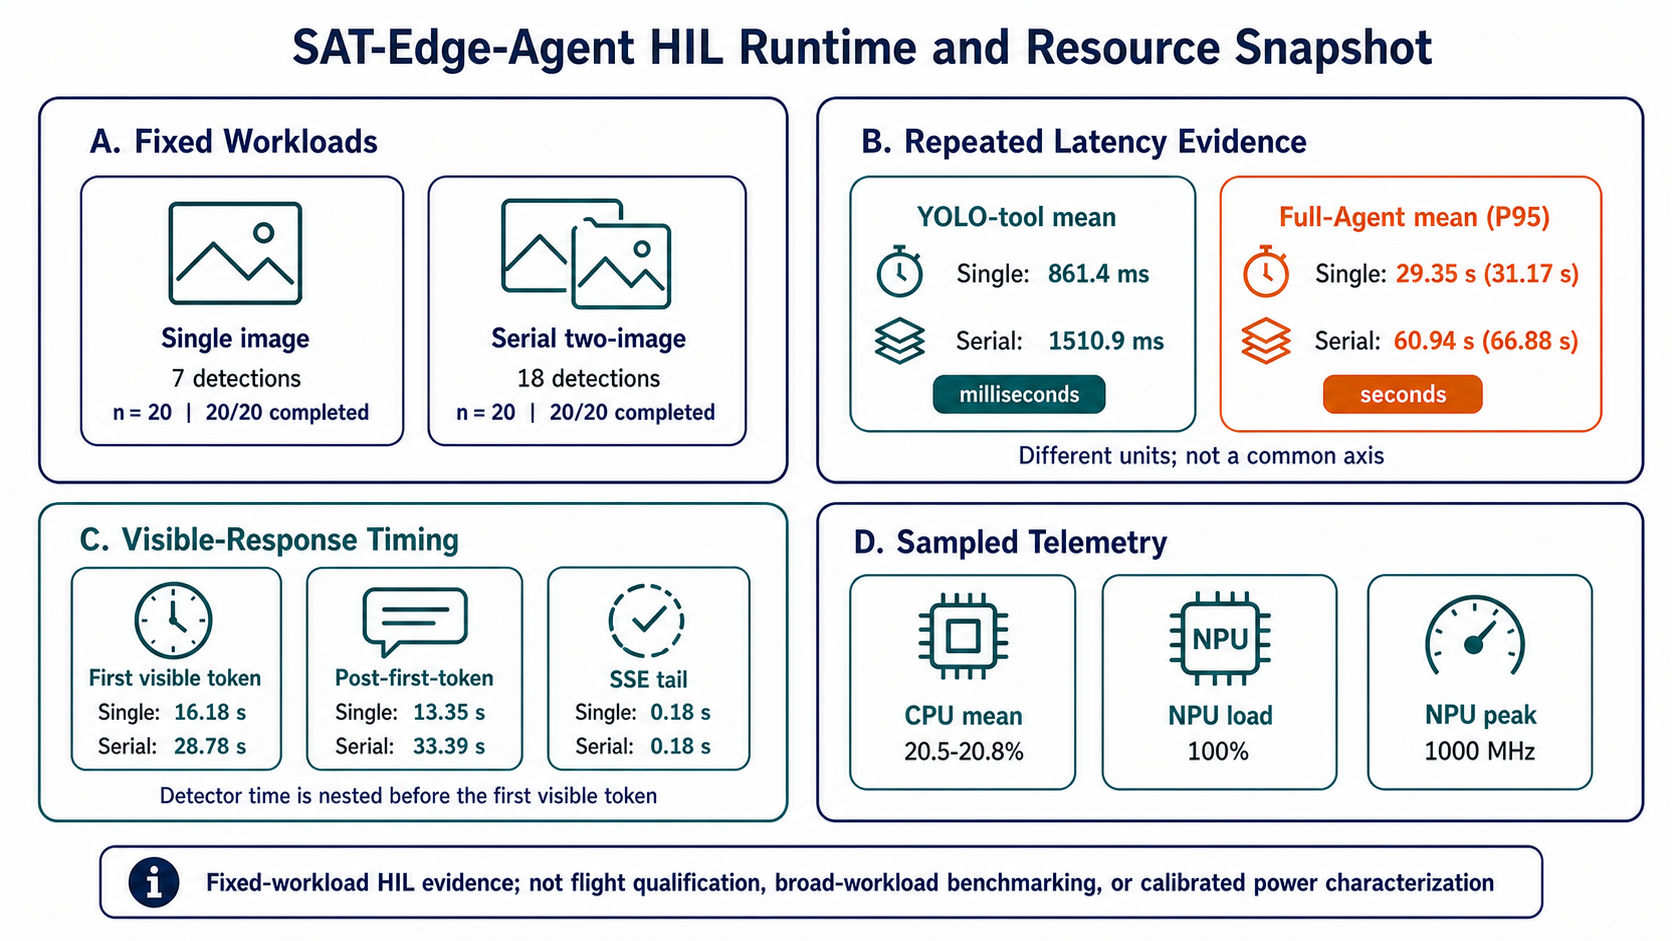
\includegraphics[width=0.98\textwidth]{figures/fig3_runtime_resource_snapshot.png}
\caption{Repeated HIL evidence for the two fixed FAIR1M workloads. Panel A defines the protocol. Panel B separates mean YOLO-tool latency in milliseconds from mean and empirical-P95 full-Agent latency in seconds; the cards do not encode a common axis. Panel C reports validated profiler intervals in seconds, with detector time identified as nested before the first visible response token rather than as an additive stage. Panel D reports the 200-ms sampled shared-accelerator NPU-load field and the $20.5$--$20.8\%$ range of the two per-workload mean CPU values. The separate 2026-07-03 plug-meter pilot is intentionally excluded.}
\label{fig:runtime_resource_snapshot}
\end{figure*}

\begin{table}[htbp]
\centering
\small
\renewcommand{\arraystretch}{1.12}
\setlength{\tabcolsep}{4pt}
\caption{Repeated full-Agent, YOLO-tool, and sampled resource statistics for the fixed FAIR1M workloads ($n=20$ each). Resource fields were sampled every 200 ms across the full request. CPU peak is the maximum observed per-request peak field, not a platform limit; the NPU field is not detector-only occupancy.}
\label{tab:agent_runtime_resource}
\begin{tabular}{p{0.43\linewidth}p{0.23\linewidth}p{0.23\linewidth}}
\toprule
\rowcolor{gray!12}
\textbf{Metric} & \textbf{Single image} & \textbf{Serial two-image} \\
\midrule
Observed completion & 20/20 & 20/20 \\
\rowcolor{graybg}
Full-Agent mean $\pm$ sample SD & $29.353 \pm 1.613$ s & $60.937 \pm 3.512$ s \\
Full-Agent median & 29.030 s & 61.134 s \\
\rowcolor{graybg}
Full-Agent empirical P95 & 31.166 s & 66.882 s \\
Full-Agent range & 26.919--34.504 s & 54.379--68.263 s \\
\rowcolor{graybg}
YOLO-tool mean $\pm$ sample SD & $861.386 \pm 11.778$ ms & $1510.920 \pm 18.180$ ms \\
YOLO-tool median & 863.415 ms & 1513.604 ms \\
\rowcolor{graybg}
YOLO-tool empirical P95 & 876.657 ms & 1535.151 ms \\
Detector share of mean Full-Agent latency & 2.93\% & 2.48\% \\
\rowcolor{graybg}
Mean sampled CPU utilization & 20.761\% & 20.482\% \\
Maximum observed CPU peak field & 86.335\% & 87.742\% \\
\rowcolor{graybg}
Mean 200-ms sampled NPU-load field & 100\% & 100\% \\
Peak sampled NPU frequency & 1000 MHz & 1000 MHz \\
\bottomrule
\end{tabular}
\end{table}

The repeated measurements show that detector execution is a small, workload-bounded fraction of the end-to-end request. It accounts for 2.93\% of the single-image mean and 2.48\% of the serial two-image mean. This finding does not imply that every remaining interval is pure language-model generation. The full-Agent window also includes Agent decisions, request construction, tool-result handling, annotated-output production, and response streaming. Likewise, the 100\% sampled NPU field does not imply continuous detector execution because the field covers shared accelerator activity over the complete request.

\subsection{Validated Visible-Response Timeline}

A separate profiler-enabled run set captures the event order \texttt{start} $\rightarrow$ \texttt{tool} $\rightarrow$ \texttt{token} $\rightarrow$ \texttt{done}. All 20 single-image profiler attempts completed. Nineteen serial two-image attempts completed both images; one additional attempt produced the structured 1/2 partial result described in the workflow section and is excluded from the all-images-successful timing mean. Table~\ref{tab:response_timeline} uses only fields validated against the raw SSE captures.

\begin{table}[htbp]
\centering
\small
\renewcommand{\arraystretch}{1.13}
\setlength{\tabcolsep}{4pt}
\caption{Mean response-timeline intervals for successful profiler-enabled runs. ``First visible token'' is an end-to-end user-visible boundary that includes pre-output Agent and tool activity; it is not pure LLM first-token latency. Detector time is nested inside that interval and must not be added to the other rows.}
\label{tab:response_timeline}
\begin{tabular}{p{0.43\linewidth}p{0.23\linewidth}p{0.23\linewidth}}
\toprule
\rowcolor{gray!12}
\textbf{Metric} & \textbf{Single image} & \textbf{Serial two-image} \\
\midrule
All-images-successful attempts & 20 & 19 \\
\rowcolor{graybg}
Full-Agent mean & 29.713 s & 62.362 s \\
Time to first visible response token & 16.184 s & 28.785 s \\
\rowcolor{graybg}
Post-first-token generation interval & 13.347 s & 33.392 s \\
SSE tail after final token & 0.182 s & 0.185 s \\
\rowcolor{graybg}
Detector-total mean (nested) & 0.857 s & 1.506 s \\
\bottomrule
\end{tabular}
\end{table}

The component CSV also contains batch HTTP, decode, inference, and annotation/render substage fields. Audit against all raw serial-batch captures found a systematic factor-of-two aggregation defect in those fields, so they are excluded from the manuscript. The validated timeline supports a narrower conclusion: most user-facing latency lies outside detector execution, both before and after the first visible token, and optimization should target the broader Agent and response-formation path.

\subsection{End-to-End Reproducibility Matrix}

Table~\ref{tab:repro_matrix} separates what a reader can reproduce directly from what remains private or replaceable. This distinction is important because the detector weight and private edge host are not the scientific contribution of the present paper.

\begin{table}[htbp]
\centering
\renewcommand{\arraystretch}{1.16}
\setlength{\tabcolsep}{4pt}
\caption{Reproducibility boundary for the SAT-Edge-Agent HIL system paper.}
\label{tab:repro_matrix}
\begin{tabular}{p{0.28\linewidth}p{0.28\linewidth}p{0.30\linewidth}}
\toprule
\rowcolor{gray!12}
\textbf{Layer} & \textbf{Publicly reproducible} & \textbf{Boundary or substitute path} \\
\midrule
Frontend/backend code & Build and run workflow, API routes, SSE stream contract & Private hostnames and paths are sanitized \\
\rowcolor{graybg}
Vision-tool contract & Health, model-status schema, success/failure JSON examples & Private YOLO weight can be replaced by a user-provided OBB model \\
Local LLM interface & OpenAI-compatible endpoint contract & Exact local model may be deployment-specific \\
\rowcolor{graybg}
Dataset sample & FAIR1M-style schema and license notes & FAIR1M-derived images must follow original dataset terms \\
Repeated timing evidence & Sanitized request-level CSVs, summary JSON/Markdown, recalculation script, and Figure 3 & Covers only the two declared fixed workloads \\
\rowcolor{graybg}
SSE and JSON contracts & Redacted success/failure JSON and normalized success/partial-result SSE examples & Raw identifiers, paths, base64 imagery, private labels, and operator text are omitted \\
Power evidence & Appendix-level plug-meter context and a public trace template & A synchronized calibrated trace is required before energy claims \\
\bottomrule
\end{tabular}
\end{table}

The reproducibility matrix separates public artifacts from replaceable or private components. The released package is located at \texttt{artifacts/hil\_orchestration/} and includes a SHA-256 manifest. Remaining workload-generalization, tail-latency, power, robustness, and metadata limitations are consolidated in the Limitations section and Appendix~\ref{app:artifacts} rather than repeated as a second evidence-gap table.
